\chapter{Implementación de una aplicación de mensajería}

En este capítulo voy a explicar como he desarrollado una aplicación de mensajería utilizando las herramientas vistas en la memoria.\\
Para desarrollar la aplicación he usado el lenguaje de programación \textbf{Python}. Aunque este lenguaje no es muy eficiente y consume muchos recursos, para la aplicación que he desarrollado no es necesario esto, ya que son dos programas independientes y ninguno de los dos necesita muchos recursos. Al igual que las aplicaciones vistas en el capítulo anterior, se ha seguido una arquitectura \textbf{cliente-servidor} por lo que se han diseñado dos aplicaciones distintas que se comunican entre si usando \textbf{sockets}. Una es la aplicación \textbf{Servidor}, esta no consta de interfaz gráfica y solo se tiene que ejecutar en un dispositivo. La otra aplicación es la aplicación \textbf{Cliente}, esta si consta de interfaz gráfica ya que es la que se va a utilizar como medio para escribir y leer los mensajes. Esta aplicación la tienen que ejecutar todos los usuarios que quieran usar el chat.

\section{Herramientas utilizadas}
Las herramientas que he utilizado para desarrollar la aplicación han sido las siguientes.
\begin{itemize}
	\item \textbf{Gestor de dependencias:} El gestor de tareas que he utilizado ha sido \textbf{Poetry}. Este gestor es de los más usado en Python. Está muy bien documentado y como archivo de configuración utiliza un archivo del tipo \emph{.toml} por lo que es muy fácil de configurar. 
	\item \textbf{Gestor de tareas:} El gestor de tareas que he usado ha sido \textbf{Poe the Poet}. Es un gestor de tareas de reciente aparición y permite automatizar las distintas tareas de una manera sencilla y con una fácil integración con Poetry. Me he decantado por este ya que esta muy actualizado, tiene una documentación exhaustiva y consta con una comunidad muy amplia.
	\item \textbf{Tests runner:} Para ejecutar tests he usado \textbf{Pytest}. Pytest es un framework que utiliza una sintaxis muy sencilla para hacer tests, además es muy fácil de integrar con las herramientas vistas anteriormente.
\end{itemize}
Además para hacer la interfaz he usado \textbf{Tkinter}, para las conexiones he usado la biblioteca \textbf{socket}, para obtener las funciones criptográficas para encriptar y desencriptar usando \emph{AES-128 GCM} \ref{esquemagcm} he usado la biblioteca \textbf{Crypto}. Además he usado la biblioteca \textbf{hashlib} para extender las claves y ajustarlas a los bloques usados en AES.

\section{Estructura de archivos}
A continuación voy a explicar la estructura de archivos que se ha seguido en el desarrollo de las aplicaciones cliente y servidor, indagando en lo que estos contienen y explicando las distintas clases y funciones que se han utilizado. 

\subsection{Cliente}
Este programa consta de dos clases, diversos métodos y funciones repartidas en los siguientes archivos. 
\begin{itemize}
	\item \textbf{src/cliente/biblioteca\textunderscore cliente.py:} En este archivo se encuentran todas las funciones necesarias para encriptar y desencriptar los mensajes.
		\begin{itemize}
			\item \textbf{SERVER\textunderscore IP}, variable en la que se almacenará la ip del servidor. Por defecto y como para las pruebas se ha ejecutado en local, tiene el valor \textbf{127.0.0.1}.
			\item \textbf{SERVER\textunderscore PORT}, variable que almacena el puerto del servidor por el que se comunicará la aplicación, tiene el valor \textbf{3333}.
			\item \textbf{rellenar\textunderscore bloque(mensaje)}, función que recibe como entrada un mensaje y lo amplia para que tenga un tamaño múltiplo de 16.
			\item \textbf{vaciar\textunderscore bloque(mensaje)}, función que recibe como entrada un mensaje y elimina los espacios en blanco añadidos para aumentar su tamaño.
			\item \textbf{encriptar(mensaje,passw)}, función que recibe como parámetros de entrada un mensaje y una contraseña, y encripta los mensajes usando \emph{AES-128} con el modo \emph{GCM}. Para poder recibir cualquier contraseña como entrada se amplia la contraseña usando una función resumen. La función devuelve tres valores: el mensaje cifrado, el nonce resultante del cifrado y tag, una etiqueta que se utiliza para asegurarse al desencriptar que el mensaje no ha sido manipulado.
			\item \textbf{desencriptar(mensaje\textunderscore cifrado, passw, tag, nonce)}, función que recibe un mensaje, una contraseña, una etiqueta y un nonce, y devuelve el mensaje desencriptado.
		\end{itemize}
	\item \textbf{src/cliente/interfaz.py:} En este archivo se encuentran las clases con sus respectivos modos para ejecutar el programa usando Tkinter.
		\begin{itemize}
			\item \textbf{Clase Ventana1}, esta clase cuenta con los métodos \textbf{enviar} y \textbf{get\textunderscore mensaje}, estos se usan para enviar y recibir mensajes a través de sockets. Además cuenta con diversos atributos en los cuales se almacenan todos los objetos usados en la interfaz como son: \textbf{server\textunderscore socket} para almacenar el socket para conectarse al servidor, \textbf{txt} donde se imprimirán los mensajes y \textbf{entrada} por donde se introducirán los mensajes para enviarlos entre otros. Esta es la ventana principal de la aplicación.
			\item \textbf{Clase Ventana2}, esta  clase cuenta con un solo método que servirá para recuperar los datos introducidos por el usuario y enviarlos al servidor, una vez hecho esto elimina la instacia actual y crea una nueva de la clase Ventana2.
					Además cuenta con diversos atributos necesarios para almacenar la información como son los atributos \textbf{emisor} que almacena el nombre de usuario o \textbf{receptor} que almacena el usuario con el que se intercambiarán los mensajes.
		\end{itemize}
	\item \textbf{src/cliente/cliente.py:} En este archivo se encuentra el programa principal, crea una instancia de la clase Ventana2 y crea un socket para conectarse con el servidor.
\end{itemize}

\subsection{Servidor}
Este programa es más sencillo que el programa cliente, ya que como he mencionado anteriormente, no consta de interfaz gráfica. Además, como la aplicación la he diseñado para que tenga un cifrado extremo a extremo no interviene en el encriptado y desencriptado de los mensajes. Consta de solo dos archivos y no tiene ninguna clase.
\begin{itemize}
	\item \textbf{src/servidor/servidor.py:} Es el programa principal y lo que hace es crear un socket por el que se conectaran todos los clientes, una función llamada \textbf{escuchar\textunderscore clientes} que se encarga de cada vez que recibe un mensaje, lo fragmenta y obtiene el emisor, el receptor, el mensaje encriptado y la etiqueta y el nonce usados en AES-128 con el modo GCM. Una vez fragmentado el mensaje se envia al usuario receptor. A continuación se crea un \textbf{Thread} con la función anterior para paralelizar la entrada de mensajes y el envío.
	\item \textbf{src/servidor/biblioteca\textunderscore servidor.py:} Archivo en el que se almacenan algunas variables globales del programa, las más importantes son: \textbf{SERVER\textunderscore IP} variable que almacena la dirección del servidor, como se ejecuta en local, en este caso \textbf{0.0.0.0} y la variable \textbf{SERVER\textunderscore PORT}, variable que almacena el puerto que se va a usar y por defecto vale \textbf{3333}.
\end{itemize}

\subsection{Mensaje}
Para codificar los mensajes he usado un string separando cada bloque con un substring llamado \textbf{separador} que vale \textless-\textgreater. El mensaje tiene la siguiente estructura.

\begin{figure}[htb]
	\centering
	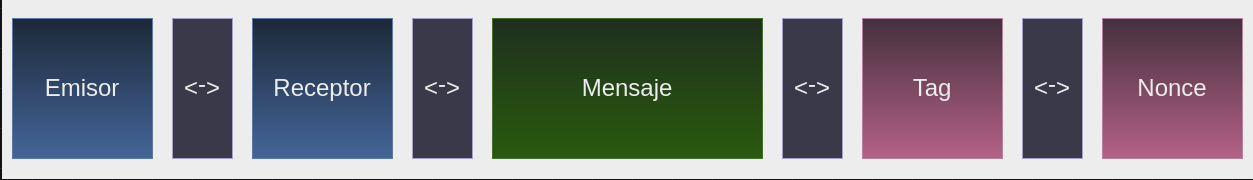
\includegraphics[width=400]{imagenes/mensaje_app.png} 
	\caption{Esquema de la codificación del mensaje.}
	\label{mensajeapp}
\end{figure}
Donde \emph{emisor} es el identificador del usuario que envía los mensajes, \emph{receptor} es el identificador del usuario que los recibe, \emph{mensaje} es el mensaje que se envía, \emph{tag} es la etiqueta usada en AES-128 con el modo GCM para validar los mensajes y \emph{nonce} es un número arbitrario que se usa solo una vez para garantizar la seguridad del mensaje frente ataques \emph{playback}. 

\section{Funcionamiento de la aplicación}
Para ejecutar la aplicación, primero se tiene que ejecutar el servidor en algún dispositivo y mientras esté en funcionamiento, ejecutar el cliente.\\
Para lanzar ambas aplicaciones hay que ejecutar el comando \emph{poe run}. Una vez ejecutado el cliente nos sale la primera interfaz donde introducimos el nombre de usuario con el que nos vamos a identificar y el nombre del usuario con el que nos vamos a comunicar \ref{appprimeraparte}.

\begin{figure}[thb]
	\centering
	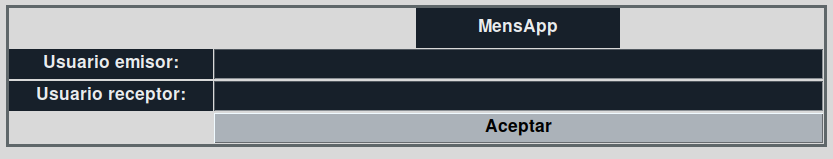
\includegraphics[width=400]{imagenes/mensapp1.png} 
	\caption{Registro en la aplicación.}
	\label{appprimeraparte}
\end{figure}
\newpage
Una vez registrados entramos en el chat con el usuario receptor. El primer mensaje que se envía, similar a otras aplicaciones de mensajería, no esta cifrado pero servirá para sincronizar ambos clientes y realizar el intercambio de claves \emph{Diffie-Hellman}. Para el intercambio he elegido como número primo 13 y como generador 2.  Una vez realizado el intercambio, que se hace de manera automática y pasa desapercibido a los usuarios, se cifran todos los mensajes. En \ref{appsegundaparte} podemos ver un ejemplo de conversación entre dos usuarios. El código de la aplicación se encuentra en un \href{https://github.com/luistf24/MensApp-TFG}{repositorio} de GitHub.
\begin{figure}[hbt]
	\centering
	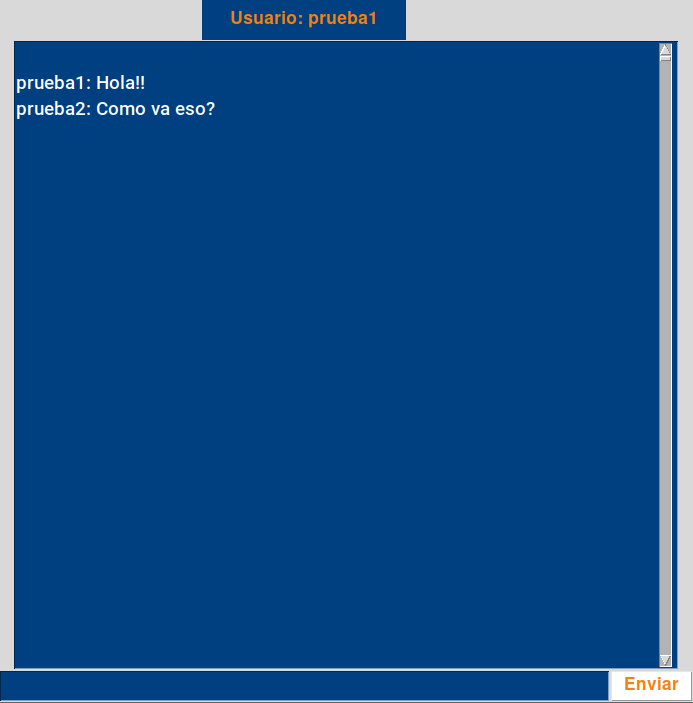
\includegraphics[scale=0.45]{imagenes/mensapp2.png} 
	\caption{Intercambio de mensajes en la aplicación.}
	\label{appsegundaparte}
\end{figure}
